\documentclass[a4paper, 11pt]{article}
\usepackage{graphicx} % Required for inserting images
\usepackage{parskip}
\usepackage[shortlabels]{enumitem}
\usepackage{geometry}
\usepackage{titling}
\usepackage{multirow}
\usepackage{verbatim}
\usepackage{array}
\usepackage{microtype}
\usepackage{changepage}
\usepackage{ragged2e}
\usepackage{longtable}
\geometry{margin=2cm}
\setlength{\arrayrulewidth}{0.5mm}
\setlength{\tabcolsep}{15pt}
\setcounter{secnumdepth}{0}
\renewcommand{\arraystretch}{1.5}
\let\newline\\



\title{GYST 5e}
\date{}
\author{}
\begin{document}
\setlength{\parskip}{6pt}
\setlength{\parindent}{12pt}
\setlist[itemize]{leftmargin=*}
\setlist[enumerate]{leftmargin=*}
\maketitle

\begin{flushright}
\textbf{Membri del team di sviluppo:}
\\Valentina Bacchelli 1021155
\\Francesco Bufalini 1028917
\end{flushright}



\newpage
\tableofcontents



\newpage
\section{Abstract}
Questo progetto propone il design di un'applicazione dedicata alla creazione e gestione di personaggi e creature nel contesto del gioco di ruolo Dungeons \& Dragons 5e. Il software mira a fornire agli utenti un ambiente intuitivo e completo per sviluppare e gestire lo stato della partita in modo automatico.

L'applicazione consente di creare i personaggi attraverso la modellazione generica dei concetti di gioco, come razza, classe e abilità, fornendo alcune opzioni predefinite disponibili per la selezione e soprattutto dando la possibilità di definirne altre a piacimento. L'applicazione permette di elaborare e modificare lo stato del gioco in seguito all'interazione da parte dell'Utente. Questo include il calcolo automatico delle statistiche, l'aggiornamento degli inventari e altro ancora, permettendo di immergersi completamente nel mondo fantastico di Dungeons \& Dragons.



\newpage
\section{Analisi dei requisiti}
\subsection{Requisiti del sistema}

\begin{enumerate}
    \item 
\end{enumerate}

\newpage
\subsubsection{Tabella dei requisiti}

\begin{center}
    \begin{tabular}{ |p{2cm}|p{8cm}|p{2cm}|  }
        \hline
        \textbf{ID} & \textbf{REQUISITO} & \textbf{TIPO} \\ 
        \hline
        R1F &  & Funzionale \\
        \hline
        ... & ... & ... \\
        \hline
    \end{tabular}
\end{center}



\newpage
\subsection{Analisi del dominio}
\subsubsection{Glossario}

\begin{center}
    \begin{tabular}{ |p{3cm}|p{8cm}|p{3cm}|  }
        \hline
        \textbf{VOCE} & \textbf{DEFINIZIONE} & \textbf{SINONIMI} \\
        \hline
        ... & ... & ... \\
        \hline
        
    \end{tabular}
\end{center}



\newpage
\subsection{Analisi dei requisiti}
\subsubsection{Casi d'uso}
\begin{figure}[h!]
    \centering
    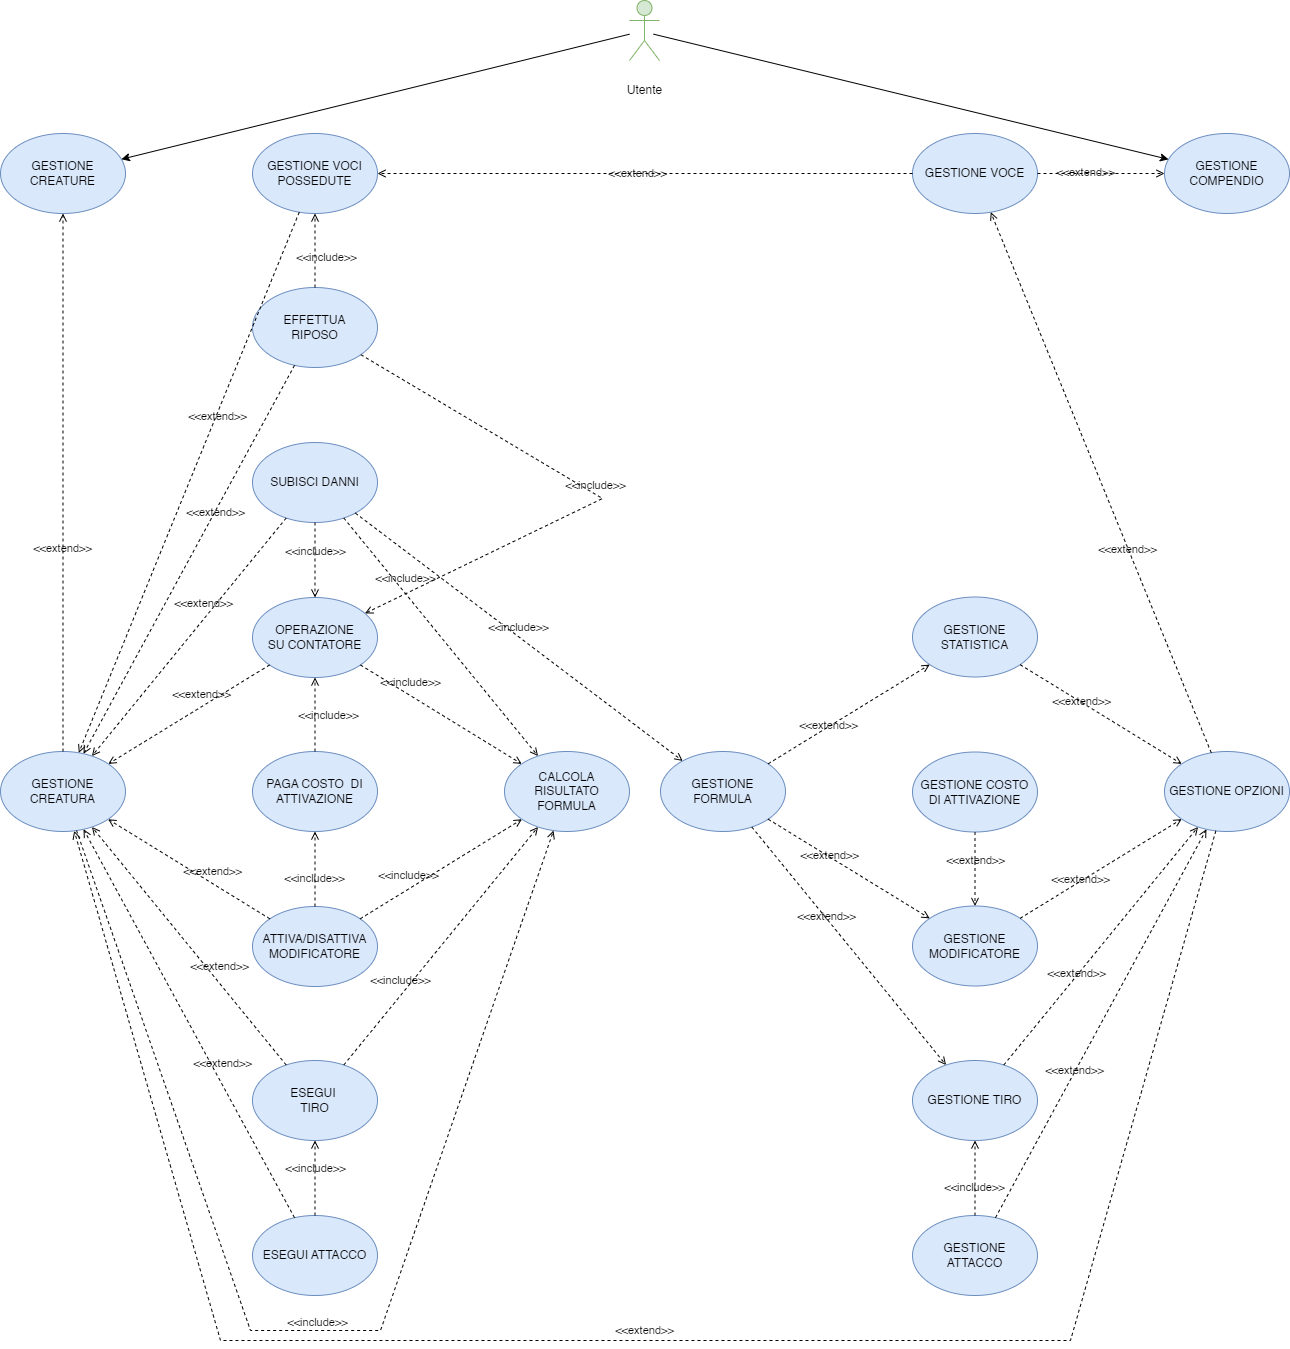
\includegraphics[width=1\textwidth,keepaspectratio]{Diagramma CU}
    \label{fig:useCase}
\end{figure}



\newpage
\subsubsection{Scenari}
\begin{center}

\begin{tabular}{ |p{5cm}|p{9.5cm}|  }
\hline
\textbf{Titolo} & Gestione Compendio \\
\hline
\textbf{Descrizione} & L'Utente visualizza e modifica le voci del suo compendio \\
\hline
\textbf{Attori} & Utente  \\
\hline
\textbf{Relazioni} & Gestione Voce \\
\hline
\textbf{Precondizioni} &  \\
\hline
\textbf{Postcondizioni} & Compendio aggiornato con le modifiche apportate \\
\hline
\textbf{Scenario principale} & 
\begin{enumerate}
    \item L'Utente seleziona la sezione di gestione del compendio
    \item Il Sistema mostra l'elenco di Voci del Compendio disponibili, divise per manuali
    \item L'Utente può visualizzarle, modificarle, aggiungerle, eliminarle, esportarle o importarne di nuove
\end{enumerate}
\\
\hline
\textbf{Scenari alternativi} & \\
\hline
    \textbf{Requisiti non funzionali} & Nel compendio non possono esistere voci duplicate e all’apertura dell’app queste vanno eliminate \\
\hline
\textbf{Punti aperti} &  \\
\hline
\end{tabular}

\vspace{3em}

\begin{tabular}{ |p{5cm}|p{9.5cm}|  }
\hline
\textbf{Titolo} & Gestione Voce \\
\hline
\textbf{Descrizione} & L'Utente visualizza una voce e ne camba gli attributi \\
\hline
\textbf{Attori} & Utente  \\
\hline
\textbf{Relazioni} & Gestione Compendio; Gestione Voci Possedute; Gestione Opzioni \\
\hline
\textbf{Precondizioni} &  \\
\hline
\textbf{Postcondizioni} & Voce aggiornata con le modifiche apportate \\
\hline
\textbf{Scenario principale} & 
\begin{enumerate}
    \item L'Utente sceglie una voce da una lista
    \item L'Utente la visualizza e può modificarne li attributi a piacimento, oppure entrare nella sezione opzioni della voce
\end{enumerate}
\\
\hline
\textbf{Scenari alternativi} & \\
\hline
    \textbf{Requisiti non funzionali} & Se viene modificata una voce attualmente usata da una creatura va mantenuta la versione pre-modifica della voce nel compendio \\
\hline
\textbf{Punti aperti} &  \\
\hline
\end{tabular}

\vspace{3em}

\begin{tabular}{ |p{5cm}|p{9.5cm}|  }
\hline
\textbf{Titolo} & Gestione Opzioni \\
\hline
\textbf{Descrizione} & L'Utente visualizza e modifica le opzioni definite in una voce o in una creatura \\
\hline
\textbf{Attori} & Utente  \\
\hline
\textbf{Relazioni} & Gestione Voce, Gestione Creatura \\
\hline
\textbf{Precondizioni} &  \\
\hline
\textbf{Postcondizioni} & Opzioni aggiornate con le modifiche apportate \\
\hline
\textbf{Scenario principale} & 
\begin{enumerate}
    \item L'Utente visualizza una lista di statistiche, modificatori, attacchi e tiri
    \item L'Utente aggiunge o rimuove un'opzione
\end{enumerate}
\\
\hline
\textbf{Scenari alternativi} & \\
\hline
    \textbf{Requisiti non funzionali} & \\
\hline
\textbf{Punti aperti} &  \\
\hline
\end{tabular}

\vspace{3em}

\begin{tabular}{ |p{5cm}|p{9.5cm}|  }
\hline
\textbf{Titolo} & Gestione Statistica \\
\hline
\textbf{Descrizione} & L'Utente visualizza e modifica una statistica definita in una voce o in una creatura \\
\hline
\textbf{Attori} & Utente  \\
\hline
\textbf{Relazioni} & Gestione Opzioni; Gestione Formula \\
\hline
\textbf{Precondizioni} &  \\
\hline
\textbf{Postcondizioni} & Statistica aggiornata con le modifiche apportate \\
\hline
\textbf{Scenario principale} & 
\begin{enumerate}
    \item L'Utente visualizza una statistica
    \item L'Utente ne cambia il nome o la formula
\end{enumerate}
\\
\hline
\textbf{Scenari alternativi} & Il nome corrisponde a quello di un'altra opzione posseduta dalla creatura e ne viene richiesta la modifica\\
\hline
    \textbf{Requisiti non funzionali} & Non possono essere definite due opzioni con lo stesso nome\\
\hline
\textbf{Punti aperti} &  \\
\hline
\end{tabular}

\vspace{3em}

\begin{tabular}{ |p{5cm}|p{9.5cm}|  }
\hline
\textbf{Titolo} & Gestione Modificatore \\
\hline
\textbf{Descrizione} & L'Utente visualizza e modifica un modificatore definito in una voce o in una creatura \\
\hline
\textbf{Attori} & Utente  \\
\hline
\textbf{Relazioni} & Gestione Opzioni; Gestione Formula \\
\hline
\textbf{Precondizioni} &  \\
\hline
\textbf{Postcondizioni} & Modificatore aggiornato con le modifiche apportate \\
\hline
\textbf{Scenario principale} & 
\begin{enumerate}
    \item L'Utente visualizza un modificatore
    \item L'Utente ne cambia gli attributi o la formula
\end{enumerate}
\\
\hline
\textbf{Scenari alternativi} &Il nome corrisponde a quello di un'altra opzione posseduta dalla creatura e ne viene richiesta la modifica \\
\hline
    \textbf{Requisiti non funzionali} &  Non possono essere definite due opzioni con lo stesso nome \\
\hline
\textbf{Punti aperti} &  \\
\hline
\end{tabular}

\vspace{3em}

\begin{tabular}{ |p{5cm}|p{9.5cm}|  }
\hline
\textbf{Titolo} & Gestione Costo di Attivazione \\
\hline
\textbf{Descrizione} & L'Utente visualizza e modifica un costo di attivazione definito in un modificatore \\
\hline
\textbf{Attori} & Utente  \\
\hline
\textbf{Relazioni} & Gestione Modificatore \\
\hline
\textbf{Precondizioni} &  \\
\hline
\textbf{Postcondizioni} & Costo aggiornato con le modifiche apportate \\
\hline
\textbf{Scenario principale} & 
\begin{enumerate}
    \item L'Utente visualizza un costo di attivazione
    \item L'Utente ne cambia gli attributi
\end{enumerate}
\\
\hline
\textbf{Scenari alternativi} & \\
\hline
    \textbf{Requisiti non funzionali} & \\
\hline
\textbf{Punti aperti} &  \\
\hline
\end{tabular}

\vspace{3em}

\begin{tabular}{ |p{5cm}|p{9.5cm}|  }
\hline
\textbf{Titolo} & Gestione Tiro \\
\hline
\textbf{Descrizione} & L'Utente visualizza e modifica un tiro definito in una voce o in una creatura \\
\hline
\textbf{Attori} & Utente  \\
\hline
\textbf{Relazioni} & Gestione Opzioni; Gestione Formula \\
\hline
\textbf{Precondizioni} &  \\
\hline
\textbf{Postcondizioni} & Tiro aggiornato con le modifiche apportate \\
\hline
\textbf{Scenario principale} & 
\begin{enumerate}
    \item L'Utente visualizza un tiro
    \item L'Utente ne cambia il tipo o la formula nel caso dei tiri con formula personalizzata
\end{enumerate}
\\
\hline
\textbf{Scenari alternativi} &Il nome corrisponde a quello di un'altra opzione posseduta dalla creatura e ne viene richiesta la modifica \\
\hline
    \textbf{Requisiti non funzionali} & Non possono essere definite due opzioni con lo stesso nome \\
\hline
\textbf{Punti aperti} &  \\
\hline
\end{tabular}

\vspace{3em}

\begin{tabular}{ |p{5cm}|p{9.5cm}|  }
\hline
\textbf{Titolo} & Gestione Attacco \\
\hline
\textbf{Descrizione} & L'Utente visualizza e modifica un attacco definito in una voce o in una creatura \\
\hline
\textbf{Attori} & Utente  \\
\hline
\textbf{Relazioni} & Gestione Opzioni\\
\hline
\textbf{Precondizioni} &  \\
\hline
\textbf{Postcondizioni} & Attacco aggiornato con le modifiche apportate \\
\hline
\textbf{Scenario principale} & 
\begin{enumerate}
    \item L'Utente visualizza un attacco
    \item L'Utente ne cambia i tiri utilizzati
\end{enumerate}
\\
\hline
\textbf{Scenari alternativi} &Il nome corrisponde a quello di un'altra opzione posseduta dalla creatura e ne viene richiesta la modifica \\
\hline
    \textbf{Requisiti non funzionali} & Non possono essere definite due opzioni con lo stesso nome \\
\hline
\textbf{Punti aperti} &  \\
\hline
\end{tabular}

\vspace{3em}

\begin{tabular}{ |p{5cm}|p{9.5cm}|  }
\hline
\textbf{Titolo} & Gestione Formula \\
\hline
\textbf{Descrizione} & L'Utente visualizza, crea o modifica una formula \\
\hline
\textbf{Attori} & Utente  \\
\hline
\textbf{Relazioni} & Gestione Statistica; Gestione Tiro; Gestione Modificatore; Subisci Danni \\
\hline
\textbf{Precondizioni} &  \\
\hline
\textbf{Postcondizioni} & Formula aggiornata e validata \\
\hline
\textbf{Scenario principale} & 
\begin{enumerate}
    \item L'Utente crea una formula o ne sceglie una
    \item L'Utente visualizza la formula
    \item L'Utente la modifica
\end{enumerate}
\\
\hline
\textbf{Scenari alternativi} &La formula è in un formato invalido per il tipo di opzione o referenzia se stessa se definita da una statistica e quindi va modificata prima di uscire \\
\hline
    \textbf{Requisiti non funzionali} & La Formula di una Statistica non può referenziare la statistica che la definisce; Una Formula deve essere in un formato che ridia un singolo intero come risultato se calcolata \\
\hline
\textbf{Punti aperti} &  \\
\hline
\end{tabular}

\vspace{3em}

\begin{tabular}{ |p{5cm}|p{9.5cm}|  }
\hline
\textbf{Titolo} & Gestione Creature Possedute \\
\hline
\textbf{Descrizione} & L'Utente visualizza e gestisce le creature nella sua lista \\
\hline
\textbf{Attori} & Utente  \\
\hline
\textbf{Relazioni} & Gestione Creatura\\
\hline
\textbf{Precondizioni} &  \\
\hline
\textbf{Postcondizioni} & Lista delle creature aggiornata \\
\hline
\textbf{Scenario principale} & L'Utente visualizza le creature disponibili e le gestisce secondo le sue esigenze potendo:
\begin{enumerate}
    \item Crearle
    \item Eliminarle
    \item Gestirle
    \item Duplicarle
    \item Importarle
    \item Esportarle
\end{enumerate} \\
\hline
\textbf{Scenari alternativi} & \\
\hline
\textbf{Requisiti non funzionali} & Devono poter esistere creature duplicate\\
\hline
\textbf{Punti aperti} & \\
\hline
\end{tabular}

\vspace{3em}

\begin{tabular}{ |p{5cm}|p{9.5cm}|  }
\hline
\textbf{Titolo} & Gestione Creatura \\
\hline
\textbf{Descrizione} & L'Utente gestisce una creatura fra quelle possedute \\
\hline
\textbf{Attori} & Utente \\
\hline
\textbf{Relazioni} & Gestione Creature; Gestione Voci Possedute; Effettua Riposo; Subisci Danni; Operazione Su Contatore; Attiva/Disattiva Modificatore; Esegui Attacco; Esegui Tiro; Calcola Risultato Formula; Gestione Opzioni \\
\hline
\textbf{Precondizioni} & \\
\hline
\textbf{Postcondizioni} & Salvato nuovo stato della Creatura\\
\hline
\textbf{Scenario principale} & L'Utente entra nell'interfaccia di gestione di una creatura dove gli vengono mostrati:
\begin{enumerate}
    \item Le informazioni base della creatura (nome e allineamento)
    \item La sezione per gestire le sue voci possedute
    \item Le statistiche che possiede con il loro valore sia come formula che come risultato
    \item I tiri disponibili per la creatura e le formule corrispondenti
    \item I modificatori posseudti dalla creatura e se sono attivi o no
\end{enumerate} \\
\hline
\textbf{Scenari alternativi} & \\
\hline
\textbf{Requisiti non funzionali} & \\
\hline
\textbf{Punti aperti} &  \\
\hline
\end{tabular}

\vspace{3em}

\begin{tabular}{ |p{5cm}|p{9.5cm}|  }
\hline
\textbf{Titolo} & Gestione Voci Possedute \\
\hline
\textbf{Descrizione} & L'Utente visualizza e gestisce le voci del compendio possedute da una creatura \\
\hline
\textbf{Attori} & Utente \\
\hline
\textbf{Relazioni} & Gestione Creatura; Gestione Effetti \\
\hline
\textbf{Precondizioni} & Creatura rispetta vincoli su quante Voci del Compendio può possedere per ogni Tipo \\
\hline
\textbf{Postcondizioni} & Lista di voci possedute della creatura aggiornata \\
\hline
\textbf{Scenario principale} & 
\begin{enumerate}
    \item L'Utente accede alla sezione di gestione delle voci possedute
    \item L'Utente ha l'opzione di aggiungere voci, rimuoverle, sostituirle. In più da qui si scelgono i privilegi selezionati per ogni voce e si possono cambiare il livello di una classe o la quantità di un oggetto
\end{enumerate}\\
\hline
\textbf{Scenari alternativi} & \\
\hline
\textbf{Requisiti non funzionali} & Una Voce del Compendio non può essere presa due volte dalla stessa Creatura\\
\hline
\textbf{Punti aperti} & \\
\hline
\end{tabular}

\vspace{3em}

\begin{tabular}{ |p{5cm}|p{9.5cm}|  }
\hline
\textbf{Titolo} & Effettua Riposo \\
\hline
\textbf{Descrizione} & La Creatura dell'Utente fa un riposo lungo o corto innescando la scelta dei privilegi e il reset dei contatori \\
\hline
\textbf{Attori} & Utente \\
\hline
\textbf{Relazioni} & Gestione Creatura; Operazione su Contatore; Gestione Voci Possedute \\
\hline
\textbf{Precondizioni} & \\
\hline
\textbf{Postcondizioni} & I contatori che dichiarano il tipo di riposo effettuato sono resettati ed è stata rieffettuata la selezione dei privilegi che si ripetono al riposo\\
\hline
\textbf{Scenario principale} & 
\begin{enumerate}
    \item L'Utente dichiara di voler effettuare un riposo
    \item L'Utente seleziona il tipo di riposo che effettua
    \item I contatori vengono aggiornati se il reset avviene al riposo scelto
    \item Viene proposto di ripetere la selezione dei privilegi per le voci interessate al riposo
\end{enumerate}\\
\hline
\textbf{Scenari alternativi} & \\
\hline
\textbf{Requisiti non funzionali} & \\
\hline
\textbf{Punti aperti} & \\
\hline
\end{tabular}

\vspace{3em}

\begin{tabular}{ |p{5cm}|p{9.5cm}|  }
\hline
\textbf{Titolo} & Subisci Danni \\
\hline
\textbf{Descrizione} & L'Utente fa prendere danni alla creatura portando una riduzione dei suoi punti vita \\
\hline
\textbf{Attori} & Utente \\
\hline
\textbf{Relazioni} & Gestione Creatura; Gestione Formula; Operazione su Contatore; Calcola Risultato Formula \\
\hline
\textbf{Precondizioni} & \\
\hline
\textbf{Postcondizioni} & I punti vita della creatura vengono ridotti \\
\hline
\textbf{Scenario principale} & 
\begin{enumerate}
    \item L'Utente dichiara di voler prendere danni
    \item L'Utente seleziona il tipo di danno che prende
    \item L'Utente immette una formula, anche con lanci di dado, che corrisponde ai danni presi
    \item L'applicazione controlla quali modificatori si applicano in base al tipo di danno
    \item L'Utente attiva o disattiva i modificatori applicati secondo le sue esigenze
    \item L'Utente conferma i valori immessi
    \item Viene calcolato il risultato della formula dopo aver applicato i modificatori attivi
    \item Viene sottratto il risultato dai Punti Ferita Temporanei della Creatura fino a portarli a 0
    \item Viene sottratto l'avanzo dai Punti Ferita Attuali
\end{enumerate}\\
\hline
\textbf{Scenari alternativi} & L'utente non conferma i danni e si ritorna all'interfaccia della gestione creatura\\
\hline
\textbf{Requisiti non funzionali} & I danni presi devono sempre essere positivi \\
\hline
\textbf{Punti aperti} & \\
\hline
\end{tabular}

\vspace{3em}

\begin{tabular}{ |p{5cm}|p{9.5cm}|  }
\hline
\textbf{Titolo} & Operazione su Contatore \\
\hline
\textbf{Descrizione} & Viene ridotto o aumentato il valore attuale di un contatore seconfo i suoi massimo e minimo \\
\hline
\textbf{Attori} & Utente \\
\hline
\textbf{Relazioni} & Gestione Creatura; Effettua Riposo; Calcola Risultato Formula; Paga Costo di Attivazione \\
\hline
\textbf{Precondizioni} & \\
\hline
\textbf{Postcondizioni} & Il valore del contatore viene aggiornato \\
\hline
\textbf{Scenario principale} & 
\begin{enumerate}
    \item Viene selezionato il contatore e di quanto cambia il suo valore
    \item Viene visualizzato il valore aggiornato del contatore e quanto è stato effettivamente ridotto
\end{enumerate}\\
\hline
\textbf{Scenari alternativi} & \\
\hline
\textbf{Requisiti non funzionali} & \\
\hline
\textbf{Punti aperti} & \\
\hline
\end{tabular}

\vspace{3em}

\begin{tabular}{ |p{5cm}|p{9.5cm}|  }
\hline
\textbf{Titolo} & Paga Costo di Attivazione \\
\hline
\textbf{Descrizione} & Viene ridotto un contatore per attivare un modificatore, e poi sostituito nella formula del modificatore la quantità pagata, che può essere usata come variabile \\
\hline
\textbf{Attori} & Utente \\
\hline
\textbf{Relazioni} & Operazione su Contatore; Attiva/Disattiva Modificatore \\
\hline
\textbf{Precondizioni} & Si sta cercando di attivare un modificatore \\
\hline
\textbf{Postcondizioni} & Il valore del contatore viene aggiornato \\
\hline
\textbf{Scenario principale} & 
\begin{enumerate}
    \item L'Utente immette una quantità positiva se il costo non è fisso
    \item Viene visualizzato il valore del contatore pre e post pagamento
    \item L'Utente conferma di voler procedere con il pagamento
    \item Viene ridotto il contatore referenziato
    \item Viene sostituita la quantità pagata nella formula del modificatore
\end{enumerate}\\
\hline
\textbf{Scenari alternativi} & Il valore attuale del contatore è troppo piccolo per effettuare il pagamento, a questo punto ci sono due possibili sviluppi:
\begin{enumerate}
    \item L'Utente decide di procedere lo stesso col pagamento e quindi viene aumentato il contatore prima di ridurlo
    \item L'Utente annulla l'attivazione del Modificatore
\end{enumerate}\\
\hline
\textbf{Requisiti non funzionali} & \\
\hline
\textbf{Punti aperti} & \\
\hline
\end{tabular}

\vspace{3em}

\begin{tabular}{ |p{5cm}|p{9.5cm}|  }
\hline
\textbf{Titolo} & Attiva/Disattiva Modificatore \\
\hline
\textbf{Descrizione} & Viene invertito lo stato attuale di un modificatore\\
\hline
\textbf{Attori} & Utente \\
\hline
\textbf{Relazioni} & Gestione Creatura; Paga Costo di Attivazione; Calcola Risultato Formula \\
\hline
\textbf{Precondizioni} & \\
\hline
\textbf{Postcondizioni} & Costo di attivazione pagato se necessario; Aggiornamento interfaccia gestione creatura e ricalcolo dei valori delle statistiche \\
\hline
\textbf{Scenario principale} & 
\begin{enumerate}
    \item L'Utente pagato il costo di attivazione se necessario
    \item L'applicazione cambia lo stato del modificatore 
    \item L'applicazione mostra l'interfaccia di gestione della creatura aggiornata ricalcolando il valore per ogni statistica
\end{enumerate}\\
\hline
\textbf{Scenari alternativi} & \\
\hline
\textbf{Requisiti non funzionali} & \\
\hline
\textbf{Punti aperti} & \\
\hline
\end{tabular}

\vspace{3em}

\begin{tabular}{ |p{5cm}|p{9.5cm}|  }
\hline
\textbf{Titolo} & Esegui Tiro \\
\hline
\textbf{Descrizione} & L'Utente sceglie un tiro fra quelli disponibili e ne vede il risultato \\
\hline
\textbf{Attori} & Utente \\
\hline
\textbf{Relazioni} & Gestione Creatura; Esegui Attacco; Calcola Risultato Formula \\\hline
\textbf{Precondizioni} & Creato il tiro desiderato \\
\hline
\textbf{Postcondizioni} & \\
\hline
\textbf{Scenario principale} & 
\begin{enumerate}
    \item L'Utente sceglie un tiro
    \item L'applicazione controlla quali modificatori si applicano in base al tipo di danno
    \item L'Utente attiva o disattiva i modificatori applicati secondo le sue esigenze
    \item L'Utente conferma i valori immessi
    \item Viene calcolato il risultato della formula dopo aver applicato i modificatori attivi
\end{enumerate}\\
\hline
\textbf{Scenari alternativi} & L'utente non conferma il tiro e si ritorna all'interfaccia della gestione creatura\\
\hline
\textbf{Requisiti non funzionali} & \\
\hline
\textbf{Punti aperti} & \\
\hline
\end{tabular}

\vspace{3em}

\begin{tabular}{ |p{5cm}|p{9.5cm}|  }
\hline
\textbf{Titolo} & Esegui Attacco \\
\hline
\textbf{Descrizione} & L'Utente sceglie un attacco fra quelli disponibili e ne effettua i tiri \\
\hline
\textbf{Attori} & Utente \\
\hline
\textbf{Relazioni} & Gestione Creatura; Esegui Tiro; \\
\hline
\textbf{Precondizioni} & Creato il tiro desiderato \\
\hline
\textbf{Postcondizioni} & \\
\hline
\textbf{Scenario principale} & 
\begin{enumerate}
    \item L'Utente sceglie un attacco
    \item Viene eseguito il tiro per colpire dell'attaco
    \item Si fanno i tiri per i danni dell'attacco, ognuno con i lanci di dadi raddoppiati (laciati due volte e sommati) se con il tiro per colpire si è fatto 20 di dado (20 naturale)
\end{enumerate}\\
\hline
\textbf{Scenari alternativi} & L'utente annulla l'attacco dopo aver fatto i tiri per colpire \\
\hline
\textbf{Requisiti non funzionali} & \\
\hline
\textbf{Punti aperti} & \\
\hline
\end{tabular}

\vspace{3em}

\begin{tabular}{ |p{5cm}|p{9.5cm}|  }
\hline
\textbf{Titolo} & Calcola Risultato Formula \\
\hline
\textbf{Descrizione} & Viene scelta una formula di cui va calcolato il risultato, che viene restituito alla fine \\
\hline
\textbf{Attori} & Utente \\
\hline
\textbf{Relazioni} & Gestione Creatura; Subisci Danni; Operazione su Contatore; Attiva/Disattiva Modificatore; Esegui Tiro; \\
\hline
\textbf{Precondizioni} & La formula passata referenzia solo statistiche definite dalla creatura \\
\hline
\textbf{Postcondizioni} & \\
\hline
\textbf{Scenario principale} & 
\begin{enumerate}
    \item Vengono espanse le variabili (statistiche) usate nella formula
    \item Vengono eseguiti i lanci di dado richiesti e sostituiti nella formula
    \item Viene calcolato il risultato matematico della formula risultante
\end{enumerate}\\
\hline
\textbf{Scenari alternativi} &\\
\hline
\textbf{Requisiti non funzionali} & \\
\hline
\textbf{Punti aperti} & \\
\hline
\end{tabular}

\vspace{3em}

\end{center}

\newpage

\subsection{Analisi dei rischi}
\subsubsection*{Tabella Valutazione Beni}
\begin{center}
    \begin{tabular}{ |p{4.5cm}|p{3.5cm}|p{4cm}|  }
        \hline
        \textbf{BENE} & \textbf{VALORE} & \textbf{ESPOSIZIONE} \\
        \hline
        Dati di Gioco & Medio. Lo scopo dell’applicazione è proprio gestirli. & Media. Compromissione dell’esperienza di gioco, perdita di progressi, dubbio sulla veridicità dei dati mostrati se attacco all’integrità dei dati. \\
        \hline
        Algoritmi e meccaniche di gioco & Medio. Proprietà intellettuale e interazione con il sistema a livello più basso. & Alta. Alterazione delle meccaniche di base che possono risultare in squilibri (per esempio alterazione dell’algoritmo di Random Number Generation) e sfruttamento degli algoritmi per esecuzione di script malevoli (code injection) \\
        \hline
    \end{tabular}
\end{center}

\subsubsection*{Tabella Minacce e Controlli}
\begin{center}
    \begin{tabular}{|p{3cm}|p{3cm}|p{3cm}|p{3.5cm}|}
        \hline
         \textbf{MINACCIA} & \textbf{PROBABILITÀ} & \textbf{CONTROLLO} & \textbf{FATTIBILITÀ} \\
         \hline
         Code Injection &Alta. Interpretazione di formule definite da altri utenti con possibili intenzioni malevole.& Sanitizzazione dell'input, utilizzo di prepared statements. & Medio costo. Richiede competenze di sviluppo sicuro, ma fondamentale per la sicurezza dell'app. \\
         \hline
         Modifiche non autorizzate dagli altri giocatori ai Personaggi & Media. Un giocatore potrebbe apportare modifiche al proprio personaggio contro le regole del gioco all’insaputa degli altri. & Log condivisibile delle modifiche effettuate. & Basso costo. Già necessario per il rollback. \\
         \hline
         Manipolazione del RNG (Random Number Generator) & Bassa. Critica per la giocabilità e l'equità. & Algoritmi di RNG sicuri, log condivisibile delle azioni effettuate. & Basso costo. Fondamentale per l'integrità del gioco. \\
         \hline
         Perdita di dati & Media. Possibilità di perdita di dati critici del gioco. & Backup regolari, log delle azioni effettuate, procedure di rollback. & Medio costo. I sistemi di backup sono essenziali e spesso richiedono un investimento in hardware/software. \\
         \hline
         Ingiunzioni legali per contenuto non autorizzato & Media. Dipende dal rispetto dei diritti di proprietà intellettuale. & Filtraggio dei contenuti, politiche chiare. & Basso costo. Protezione legale e della reputazione. Sfruttamento dell’Open Game License. \\
         \hline
    \end{tabular}
\end{center}

\vspace{2em}

\subsubsection*{Analisi Tecnologica della Sicurezza}
\begin{center}
    \begin{tabular}{|p{6cm}|p{8cm}|}
        \hline
        \textbf{Tecnologia} & \textbf{Vulnerabilità} \\
        \hline
        Interprete di formule dinamiche & 
        \begin{itemize}
            \item Code Injection
        \end{itemize} \\
        
        \hline
        Generatore di numeri casuali &
        \begin{itemize}
            \item RNG Attacks
        \end{itemize}\\
        
        \hline
        Log &
        \begin{itemize}
            \item Manipolazione e non integrità dei log
        \end{itemize}\\
        \hline 
    \end{tabular}
\end{center}



\newpage



\subsubsection{Security Use Case e Misuse Case}
\begin{figure}[h!]
    \centering
    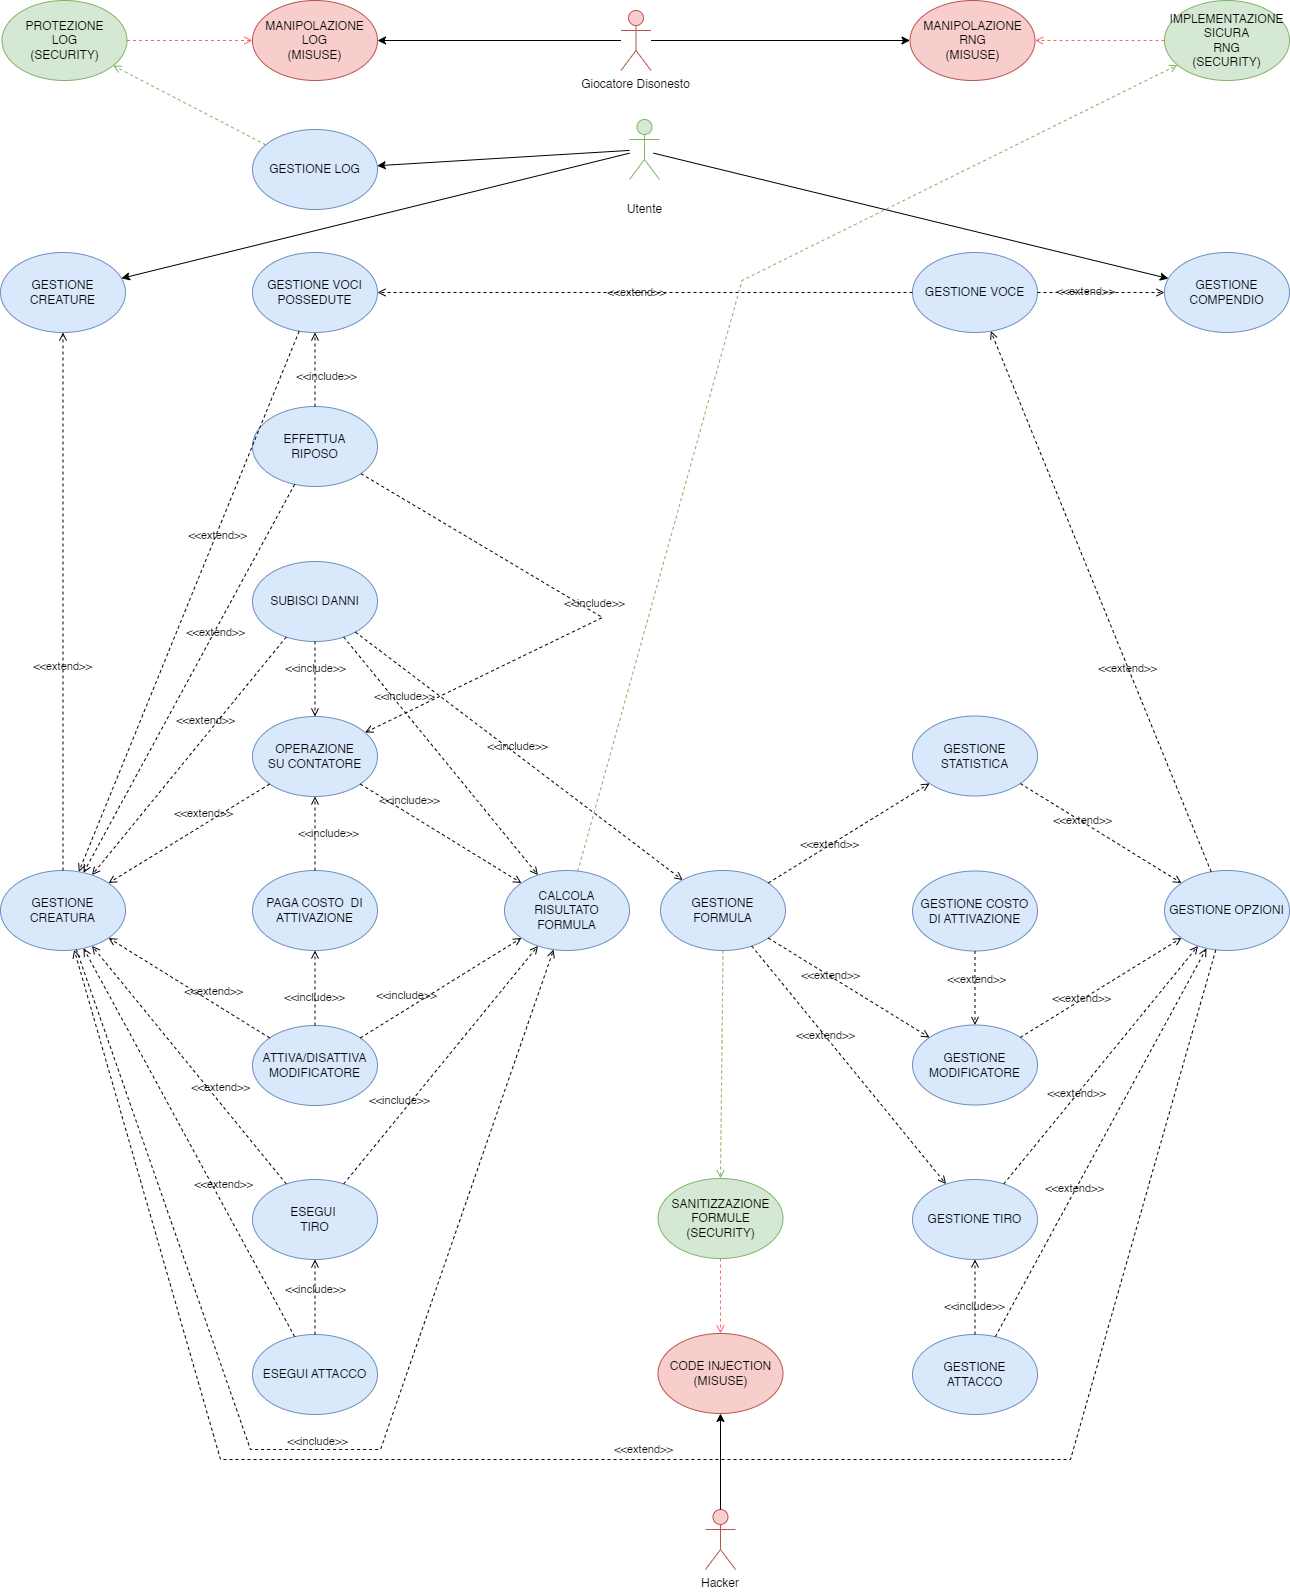
\includegraphics[width=1\textwidth,keepaspectratio]{Diagramma CU-Security}
    \label{fig:security}
\end{figure}

\newpage
\begin{table}[h]\small   
\begin{center}
\begin{tabular}{ |p{4cm}|p{11cm}|  }
\hline
\textbf{Titolo} & Protezione Log \\
\hline
\textbf{Descrizione} & I file di log devono essere protetti da manipolazioni per garantire l'integrità e la trasparenza delle operazioni \\
\hline
\textbf{Misuse case} & Manipolazione Log  \\
\hline
\textbf{Relazioni} &  \\
\hline
\textbf{Precondizioni} & L'attaccante ha un accesso parziale o ha scoperto una vulnerabilità nei file di log.  \\
\hline
\textbf{Postcondizioni} & Il sistema protegge i log in modo che ne sia verificabile l'integrità.  \\
\hline
\end{tabular}
    \begin{tabular}{|p{4cm}|p{4.9cm}|p{5cm}|}
        \multirow{3}{=}{\textbf{Scenario principale}} & \textbf{Sistema} & \textbf{Attaccante}\\\cline{2-3}
         & Protegge i file di log in modo che ne sia verificabile l'integrità. &  \\\cline{2-3}
         & & Tenta di modificare o cancellare i file di log per nascondere le sue azioni. \\\cline{2-3}
         & La non integrità dei log è visibile agli altri giocatori, che individuano il tentativo di manipolazione. & \\
         \hline
         \multirow{5}{=}{\textbf{Scenario di attacco avvenuto con successo}} & \textbf{Sistema} & \textbf{Attaccante}\\\cline{2-3}
         & Protegge i file di log in modo che ne sia verificabile l'integrità. &  \\\cline{2-3}
         && L'attaccante riesce a cancellare o alterare i log, nascondendo le tracce delle operazioni disoneste, e riesce a farli apparire integri. \\\cline{2-3}
         & Gli altri giocatori non rilevano la manipolazione dei log. & \\\cline{2-3}
         && Trae vantaggio dalle modifiche disoneste apportate a insaputa degli altri. \\
    \hline
    \end{tabular}
    \end{center}
\end{table}

\clearpage
\begin{table}[h]\small
\begin{center}
\begin{tabular}{ |p{4cm}|p{11cm}|  }
\hline
\textbf{Titolo} & Implementazione Sicura RNG \\
\hline
\textbf{Descrizione} & Il generatore di numeri casuali (RNG) deve essere sicuro e resistente a manipolazioni per garantire equità nel gioco. \\
\hline
\textbf{Misuse case} & Manipolazione RNG \\
\hline
\textbf{Relazioni} &  \\
\hline
\textbf{Precondizioni} &L'attaccante ha accesso al sistema e riesce a manipolare o prevedere il comportamento dell'RNG.\\
\hline
\textbf{Postcondizioni} & Il sistema utilizza algoritmi crittograficamente sicuri per la generazione di numeri casuali.  \\
\hline
\end{tabular}
    \begin{tabular}{|p{4cm}|p{4.9cm}|p{5cm}|}
        \multirow{5}{=}{\textbf{Scenario principale}} & \textbf{Sistema} & \textbf{Attaccante}\\\cline{2-3}
        & Il sistema utilizza un algoritmo di RNG sicuro. &\\\cline{2-3}
        & & L'attaccante tenta di influenzare o prevedere i risultati dell'RNG, ma non riesce a superare il meccanismo di protezione.\\\cline{2-3}
        & La generazione di numeri casuali rimane inalterata. &\\
        \hline
        \multirow{5}{=}{\textbf{Scenario di attacco avvenuto con successo}} & \textbf{Sistema} & \textbf{Attaccante}\\\cline{2-3}
        & Il sistema utilizza un algoritmo di RNG sicuro. & \\\cline{2-3}
        & & L'attaccante riesce a superare il meccanismo di protezione e sfrutta la manipolazione dell'RNG per ottenere risultati prevedibili o favorevoli. \\
    \hline
    \end{tabular}
\end{center}
\end{table}

\clearpage
\begin{table}[h]\small
\begin{center}
\begin{tabular}{ |p{4cm}|p{11cm}|  }
\hline
\textbf{Titolo} & Sanitizzazione Formule \\
\hline
\textbf{Descrizione} & Le formule definite dagli utenti devono essere sanitizzate per prevenire code injection. \\
\hline
\textbf{Misuse case} & Code Injection \\
\hline
\textbf{Relazioni} &  \\
\hline
\textbf{Precondizioni} & L’Attaccante ha i mezzi per eseguire codice malevolo attraverso la possibilità di inserire formule personalizzate fornita dall'applicazione, e le condivide ad altri utenti che le importeranno nella loro applicazione. \\
\hline
\textbf{Postcondizioni} & Il Sistema rileva e blocca l'esecuzione delle formule ritenute potenzialmente dannose. \\
\hline
\end{tabular}
    \begin{tabular}{|p{4cm}|p{4.9cm}|p{5cm}|}
        \multirow{3}{=}{\textbf{Scenario principale}} & \textbf{Sistema} & \textbf{Attaccante}\\\cline{2-3}
        && Condivide con altri utenti formule contenenti codice malevolo, e loro le importano.\\\cline{2-3}
        & Individua il tentativo e sanitizza le formule potenzialmente dannose. & \\\cline{2-3}
         \hline
         \multirow{5}{=}{\textbf{Scenario di attacco avvenuto con successo}} & \textbf{Sistema} & \textbf{Attaccante}\\\cline{2-3}
         && Condivide con altri utenti formule contenenti codice malevolo, e loro le importano.\\\cline{2-3}
         & Non rileva la formula come potenzialmente dannosa e procede nell'esecuzione. & \\\cline{2-3}
         & La formula viene eseguita e potrebbe danneggiare il Sistema. & \\\cline{2-3}
    \hline
    \end{tabular}
\end{center}
\end{table}

\clearpage
\newpage
\subsubsection*{Requisiti di Protezione dei Dati}
Dall’analisi del rischio si possono evincere i seguenti ulteriori requisiti:
\begin{enumerate}[\indent1.]
    \item Creazione di un log per tenere traccia di tutte le azioni svolte dall’Utente.
    \item Implementazione di un sistema di sanitizzazione dell’input delle formule personalizzate per impedire l’esecuzione di codice malevolo.
    \item Individuazione di un adeguato sistema di protezione dell’integrità dei log.
\end{enumerate}

\subsubsection{Requisiti di Sistema Aggiornati}

\begin{center}
    \begin{tabular}{ |p{2cm}|p{8cm}|p{2cm}|  }
        \hline
        ID & REQUISITO & TIPO \\ 
        \hline
        R1F &  & Funzionale \\
        \hline
        ... & ... & ... \\
        \hline
    \end{tabular}
\end{center}

\subsubsection{Glossario Aggiornato}

\begin{center}
    \begin{tabular}{ |p{3cm}|p{6cm}|p{3cm}|  }
        \hline
        VOCE & DEFINIZIONE & SINONIMI \\
        \hline
        Log & Registro dove vengono salvate informazioni per tracciare le operazioni eseguite. & Registro \\
        \hline
        Voce di Log & Una singola riga di Log che rappresenta una singola azione effettuata dall'Utente & Riga di Log, Record di Log \\\hline
    \end{tabular}
\end{center}

\subsubsection{Scenari Aggiornati}

\begin{center}
    \begin{tabular}{ |p{5cm}|p{9.5cm}|  }
        \hline
        \textbf{Titolo} & Gestione Log \\
        \hline
        \textbf{Descrizione} & L'Utente visualizza i log \\
        \hline
        \textbf{Attori} & Utente \\
        \hline
        \textbf{Relazioni} & \\
        \hline
        \textbf{Precondizioni} &  \\
        \hline
        \textbf{Postcondizioni} & \\
        \hline
        \textbf{Scenario principale} & L'Utente accede alla sezione di visualizzazione log e vede l'elenco delle azioni effettuate.
        \\
        \hline
        \textbf{Scenari alternativi} & \\
        \hline
        \textbf{Requisiti non funzionali} & \\
        \hline
        \textbf{Punti aperti} &  \\
        \hline
    \end{tabular}
\end{center}


\newpage

\subsection{Descrizione delle interfacce grafiche (OPZIONALE)}

\newpage
\section{Analisi del Problema}
\subsection{Analisi delle Funzionalità}
\subsubsection*{Tabella delle funzionalità}
\begin{center}
    \begin{tabular}{|p{3cm}|p{3cm}|p{3cm}|p{3cm}|}
        \hline
        \textbf{Funzionalità} & \textbf{Tipo} & \textbf{Grado \newline Complessità} & \textbf{Requisiti \newline Collegati} \\
        \hline
        Gestione \newline Compendio & Gestione Dati, Memorizzazione Dati, Interazione con l’esterno & Complessa & \\
        \hline
        Gestione Voce & Gestione Dati, Memorizzazione Dati & Complessa & \\
        \hline
        Gestione Opzioni & Gestione Dati, Memorizzazione Dati & Complessa & \\
        \hline 
        Gestione Creature & Gestione Dati, Memorizzazione Dati, Interazione con l’esterno & Complessa & \\
        \hline
        Gestione Creatura & Gestione Dati, Memorizzazione Dati & Complessa & \\
        \hline
        Gestione Formula & Gestione Dati, Memorizzazione Dati & Semplice & \\
        \hline
        Calcola Risultato Formula & Gestione Dati & Semplice & \\
        \hline
        Gestione Log & Gestione Dati, Interazione con l'esterno & Semplice & \\\hline
    \end{tabular}
\end{center}

\vspace{2em}

\setlength{\tabcolsep}{10pt}
\subsubsection*{Gestione Compendio: Tabella Informazioni/Flusso}
\begin{adjustwidth}{-1.5cm}{-1.5cm}
\begin{center}
    \begin{tabular}{|p{3cm}|p{1.5cm}|p{3.5cm}|p{2.5cm}|p{4cm}|}
        \hline
        \textbf{Informazione} & \textbf{Tipo} & \textbf{Livello \newline Protezione/Privacy} & \textbf{Input/Output}&\textbf{Vincoli}\\
        \hline
        Nome Voce & Semplice & Protezione bassa & Output & Massimo 64 caratteri\\\hline
        
    \end{tabular}
\end{center}
\end{adjustwidth}

\clearpage
\newpage
\subsubsection*{Gestione Voce: Tabella Informazioni/Flusso}
\begin{adjustwidth}{-1.5cm}{-1.5cm}
\begin{center}
    \begin{tabular}{|p{3cm}|p{1.5cm}|p{3.5cm}|p{2.5cm}|p{4cm}|}
        \hline
        \textbf{Informazione} & \textbf{Tipo} & \textbf{Livello \newline Protezione/Privacy} & \textbf{Input/Output}&\textbf{Vincoli}\\
        \hline
        Id & Semplice & Protezione bassa & Output & Massimo 64 caratteri \\
        \hline
        Nome & Semplice & Protezione bassa & Input/Output & Massimo 64 caratteri \\
        \hline
        Descrizione & Semplice & Protezione bassa & Input/Output &  \\
        \hline
        Nome manuale & Semplice & Protezione bassa & Input/Output & Massimo 64 caratteri \\
        \hline        
        Opzioni di voce & Composto & Protezione bassa & Input/Output & \\\hline
        Numero privilegi \newline selezionabili & Semplice & Protezione bassa & Input/Output & Intero \\
        \hline
        Privilegi \newline selezionabili \newline \newline Composti da:
            \begin{itemize}
                \item Nome
                \item Descrizione
            \end{itemize}
         & Composto & Protezione bassa & Input/Output & Il nome può essere di massimo 64 caratteri\\
        \hline
    \end{tabular}
\end{center}
\end{adjustwidth}

\vspace{2em}

\subsubsection*{Gestione Opzioni: Tabella Informazioni/Flusso}
\begin{adjustwidth}{-1.5cm}{-1.5cm}
\begin{center}
    \begin{tabular}{|p{3cm}|p{1.5cm}|p{3.5cm}|p{2.5cm}|p{4cm}|}
        \hline
        \textbf{Informazione} & \textbf{Tipo} & \textbf{Livello \newline Protezione/Privacy} & \textbf{Input/Output} & \textbf{Vincoli} \\
        \hline
        Id opzione & Semplice & Protezione bassa & Output & Massimo 64 caratteri \\\hline
        Nome opzione & Semplice & Protezione bassa & Input/Output & Massimo 64 caratteri \\
        \hline
        Tiro se è un Tiro \newline \newline Composto da:
        \begin{itemize}
            \item Tipo di tiro 
            \item Caratteristica usata 
            \item Nome oggetto usato 
        \end{itemize}
        & Composto & Protezione bassa & Input/Output & \\
        \hline
        Statistica se è una Statistica \newline \newline Composta da: \begin{itemize}
            \item Valore sotto forma di Formula o Mappa di valori 
            \item Riposo e valore di reset se è un contatore
        \end{itemize} & Composto & Protezione bassa & Input/Output & \\
        \hline
        Attacco se è un Attacco \newline \newline Composto da: \begin{itemize}
            \item Tiro per colpire associato 
            \item Tiri per i Danni associati
        \end{itemize}  & Composto & Protezione bassa & Input/Output & \\
        \hline
        Modificatore se è un Modificatore \newline \newline Composto da: 
        \begin{itemize}
            \item Parola chiave per vecchia formula 
            \item Identificatore associato 
            \item Costo di Attivazione 
            \item Nuova formula
        \end{itemize} & Composto & Protezione bassa & Input/Output & La Nuova Formula è una stringa predefinita se si tratta di un modificatore non cumulabile \\
        \hline
    \end{tabular}
\end{center}
\end{adjustwidth}


\vspace{2em}

\subsubsection*{Gestione Creature: Tabella Informazioni/Flusso}
\begin{adjustwidth}{-1.5cm}{-1.5cm}
\begin{center}
    \begin{tabular}{|p{3cm}|p{1.5cm}|p{3.5cm}|p{2.5cm}|p{4cm}|}
        \hline
        \textbf{Informazione} & \textbf{Tipo} & \textbf{Livello \newline Protezione/Privacy} & \textbf{Input/Output}&\textbf{Vincoli}\\
        \hline
        Nome creatura & Semplice & Protezione bassa & Output & Massimo 64 caratteri \\\hline
    \end{tabular}
\end{center}
\end{adjustwidth}

\subsubsection*{Gestione Creatura: Tabella Informazioni/Flusso}
\begin{adjustwidth}{-1.5cm}{-1.5cm}
\begin{center}
    \begin{tabular}{|p{4cm}|p{1.5cm}|p{3cm}|p{2.5cm}|p{4cm}|}
        \hline
        \textbf{Informazione} & \textbf{Tipo} & \textbf{Livello \newline Protezione/\newline Privacy} & \textbf{Input/Output} & \textbf{Vincoli} \\
        \hline
        Id & Semplice & Protezione bassa & Output & Massimo 64 caratteri \\
        \hline
        Nome & Semplice & Protezione bassa & Input/Output & Massimo 64 caratteri \\
        \hline
        Allineamento & Semplice & Protezione bassa & Input/Output & Uno dei valori consentiti come da specifica del vocabolario \\
        \hline
        Voci Possedute \newline \newline Composte da:
        \begin{itemize}
            \item Tutte le informazioni incluse in \textbf{Gestione Voce: Tabella Informazioni/Flusso}
            \item Livello in classe (se è una classe)
            \item Quantità posseduta (se è un oggetto)
        \end{itemize}
        & Composto & Protezione bassa & Input/Output & Id, nome e nome manuale possono essere al massimo di 64 caratteri, il numero privilegi selezionabili, livello in classe e quantità posseduta devono essere interi \\
        \hline
        Opzioni di Creatura \newline \newline Composte da: 
        \begin{itemize}
            \item Tutte le informazioni incluse in \newline \textbf{Gestione Opzioni: Tabella Informazioni/Flusso}
        \end{itemize}& Composto & Protezione bassa & Input/Output &  \\
        \hline
        Statistiche \newline \newline Composte da: \begin{itemize}
            \item Nome
            \item Valore
            \item Se è un contatore, valore di reset e riposo di reset
        \end{itemize}& Composto & Protezione bassa & Input/Output & Il nome può essere al massimo di 64 caratteri, il valore e il valore di reset sono interi \\
        \hline
    \end{tabular}
    \begin{tabular}{|p{3.5cm}|p{1.5cm}|p{3.5cm}|p{2.5cm}|p{4cm}|}
    \hline
        Tiri disponibili \newline \newline Composti da:
        \begin{itemize}
            \item Nome
            \item Tipo di tiro
            \item Caratteristica usata
            \item Nome oggetto usato
            \item Formula
            \item Tipo di Danno (se è un Tiro per i Danni)
            \item Tipo di Attacco (se è un Tiro per Colpire)
            \item Abilità usata (e se si tratta di una Prova di Lotta, se è una Prova Caratteristica)
        \end{itemize}& Composto & Protezione bassa & Input/Output & Nome e nome oggetto usato sono di massimo 64 caratteri. La formula deve essere una stringa valida come da specifiche dei requisiti e del vocabolario. \\
        \hline
        Modificatori posseduti \newline \newline Composti da:
        \begin{itemize}
            \item Parola chiave per vecchia formula
            \item Identificatore
            \item Costo di Attivazione
            \item Nuova formula
        \end{itemize}& Composto & Protezione bassa & Input/Output & \\
        \hline
        Attacchi disponibili \newline \newline Composti da: \begin{itemize}
            \item Tiri per Colpire associati
            \item Tiri per i Danni associati
        \end{itemize} & Composto & Protezione bassa & Input/Output &  \\
        \hline
    \end{tabular}
\end{center}
\end{adjustwidth}


\vspace{2em}

\subsubsection*{Gestione Formula: Tabella Informazioni/Flusso}
\begin{adjustwidth}{-1.5cm}{-1.5cm}
\begin{center}
    \begin{tabular}{|p{3cm}|p{1.5cm}|p{3.5cm}|p{2.5cm}|p{4cm}|}
        \hline
        \textbf{Informazione} & \textbf{Tipo} & \textbf{Livello \newline Protezione/Privacy} & \textbf{Input/Output}&\textbf{Vincoli}\\
        \hline
        Valore massimo & Semplice & Protezione bassa & Input/Output & Intero \\
        \hline
        Valore minimo & Semplice & Protezione bassa & Input/Output & Intero \\
        \hline
        Formula & Semplice &  & Input/Output & Stringa valida come da specifiche dei requisiti e del vocabolario \\
        \hline
    \end{tabular}
\end{center}
\end{adjustwidth}

\vspace{2em}

\subsubsection*{Calcola Risultato Formula: Tabella Informazioni/Flusso}
\begin{adjustwidth}{-1.5cm}{-1.5cm}
\begin{center}
    \begin{tabular}{|p{3cm}|p{1.5cm}|p{3.5cm}|p{2.5cm}|p{4cm}|}
        \hline
        \textbf{Informazione} & \textbf{Tipo} & \textbf{Livello \newline Protezione/Privacy} & \textbf{Input/Output}&\textbf{Vincoli}\\
        \hline
        Formula & Semplice & Protezione bassa & Output & Stringa valida come da specifiche dei requisiti e del vocabolario \\\hline
        Modificatori applicabili \newline \newline Composti da:
        \begin{itemize}
            \item Parola chiave per vecchia formula
            \item Identificatore
            \item Costo di Attivazione
            \item Nuova formula
        \end{itemize}& Composto & Protezione bassa & Input/Output & \\\hline
    \end{tabular}
\end{center}
\end{adjustwidth}

\vspace{2em}

\subsubsection*{Gestione Log: Tabella Informazioni/Flusso}
\begin{adjustwidth}{-1.5cm}{-1.5cm}
\begin{center}
    \begin{tabular}{|p{3cm}|p{1.5cm}|p{3.5cm}|p{2.5cm}|p{4cm}|}
        \hline
        \textbf{Informazione} & \textbf{Tipo} & \textbf{Livello \newline Protezione/Privacy} & \textbf{Input/Output}&\textbf{Vincoli}\\
        \hline
        Voce di Log \newline Composta da: \begin{itemize}
            \item Timestamp
            \item Descrizione
        \end{itemize} & Composto & Protezione alta & Output & \\\hline
    \end{tabular}
\end{center}
\end{adjustwidth}

\clearpage
\newpage
\subsection{Analisi dei Vincoli}
\subsubsection*{Tabella vincoli}
\begin{center}
    \begin{tabular}{|p{3cm}|p{3cm}|p{3.5cm}|p{3.5cm}|}
        \hline
        \textbf{Requisito} & \textbf{Categoria} & \textbf{Impatto} & \textbf{Funzionalità} \\
        \hline
        Velocità di \newline memorizzazione dei dati & Tempo di risposta & Cercare di migliorare & Gestione Compendio, Gestione Voce, \newline Gestione Opzioni, Gestione Creature, Gestione Creatura, Gestione Formula \\
        \hline
        Semplicità di navigazione nell'applicazione & Usabilità & Cercare di migliorare & Gestione Compendio, Gestione Voce, \newline Gestione Opzioni, Gestione Creature, Gestione Creatura, Gestione Formula \\
        \hline
        Ottimizzazione del tempo di aggiornamento delle interfacce al cambiamento di stato & Tempo di risposta & Cercare di migliorare & Gestione Compendio, Gestione Voce, \newline Gestione Opzioni, Gestione Creature, Gestione Creatura, Gestione Formula, Calcola Risultato Formula \\
        \hline
        Facile \newline manutenibilità ed estensione futura & Riusabilità & Peggioramento tempo di risposta, aumento del numero di entità & Gestione Compendio, Gestione Voce, \newline Gestione Opzioni, Gestione Creature, Gestione Creatura, Gestione Formula, Calcola Risultato Formula \\
        \hline
    \end{tabular}
\end{center}

\clearpage
\newpage
\subsection{Analisi delle Interazioni}
\subsubsection*{Tabella maschere}
\begin{adjustwidth}{-1.5cm}{-1.5cm}
    \begin{center}
        \begin{longtable}{|p{5cm}|p{5cm}|p{5cm}|}
        \hline
        \textbf{Maschera} & \textbf{Informazioni} & \textbf{Funzionalità} \\ \hline
        Home Compendio & 
        Navigazione verso: 
        \begin{itemize}
            \item View Crea Voce 
            \item View Elimina Voce 
            \item View Importa Voci 
            \item View Esporta Voci
        \end{itemize}
        Visualizzazione di (per ogni voce):
        \begin{itemize}
            \item View Voce
        \end{itemize} & 
        Gestione Compendio \\ \hline
        
        View Crea Voce & 
        Visualizzazione di:
        \begin{itemize}
            \item Finestra di dialogo con richiesta di conferma
            \item View Voce
        \end{itemize} & 
        Gestione Compendio \\ \hline
        
        View Elimina Voce & 
        Visualizzazione di:
        \begin{itemize}
            \item Finestra di dialogo con richiesta di conferma
        \end{itemize} & 
        Gestione Compendio \\ \hline
        
        View Importa Voci & 
        Navigazione verso:
        \begin{itemize}
            \item Esplora risorse del sistema sottostante
        \end{itemize}
        Visualizzazione di:
        \begin{itemize}
            \item Finestra di dialogo con richiesta di conferma per scelta file
        \end{itemize} & 
        Gestione Compendio \\ \hline
        
        View Esporta Voci & 
        Navigazione verso:
        \begin{itemize}
            \item Esplora risorse del sistema sottostante
        \end{itemize}
        Visualizzazione di:
        \begin{itemize}
            \item Finestra di dialogo con richiesta di conferma per scelta file
        \end{itemize} & 
        Gestione Compendio \\ \hline
        
        View Voce & 
        Navigazione verso:
        \begin{itemize}
            \item View Crea Privilegio
            \item View Elimina Privilegio
        \end{itemize}
        Visualizzazione di (per ogni privilegio selezionabile):
        \begin{itemize}
            \item View Privilegio
        \end{itemize}
        Visualizzazione di:
        \begin{itemize}
            \item Home Gestione Opzioni
        \end{itemize}
        Visualizzazione (con possibilità di modifica) di:
        \begin{itemize}
            \item Nome Manuale
            \item Nome
            \item Descrizione
            \item Innesco scelta Privilegi
            \item Numero Privilegi Selezionabili
        \end{itemize}
        Visualizzazione (con possibilità di modifica) di (se oggetto):
        \begin{itemize}
            \item Tipo oggetto
            \item Proprietà possedute
        \end{itemize} & 
        Gestione Voce \\ \hline
        
        View Crea Privilegio & 
        Visualizzazione di:
        \begin{itemize}
            \item Finestra di dialogo con richiesta di conferma
            \item View Creazione Voce
        \end{itemize} & 
        Gestione Voce \\ \hline
        
        View Elimina Privilegio & 
        Visualizzazione di:
        \begin{itemize}
            \item Finestra di dialogo con richiesta di conferma
        \end{itemize} & 
        Gestione Voce \\ \hline
        
        View Privilegio & 
        Visualizzazione di:
        \begin{itemize}
            \item View Voce
        \end{itemize}
        Visualizzazione di (se privilegio di classe):
        \begin{itemize}
            \item Classe di riferimento per livello
        \end{itemize} & 
        Gestione Voce \\ \hline
        
        Home Gestione Opzioni & 
        Navigazione verso:
        \begin{itemize}
            \item View Crea Opzione
            \item View Elimina Opzione
        \end{itemize}
        Visualizzazione di (per ogni tiro):
        \begin{itemize}
            \item View Tiro
        \end{itemize}
        Visualizzazione di (per ogni statistica):
        \begin{itemize}
            \item View Statistica
        \end{itemize}
        Visualizzazione di (per ogni attacco):
        \begin{itemize}
            \item View Attacco
        \end{itemize}
        Visualizzazione di (per ogni modificatore):
        \begin{itemize}
            \item View Modificatore
        \end{itemize} & 
        \\ \hline
        
        View Crea Opzione & 
        Richiesta di:
        \begin{itemize}
            \item Tipo opzione da creare
        \end{itemize}
        Visualizzazione di:
        \begin{itemize}
            \item Finestra di dialogo con richiesta di conferma
            \item Home Gestione Opzioni
        \end{itemize} & 
        \\ \hline
        
        View Elimina Opzione & 
        Visualizzazione di:
        \begin{itemize}
            \item Finestra di dialogo con richiesta di conferma
        \end{itemize} & 
        \\ \hline
        
        View Tiro & 
        Visualizzazione (con possibilità di modifica) di:
        \begin{itemize}
            \item Nome
            \item Tipo di tiro
            \item Caratteristica usata
            \item Nome oggetto usato
        \end{itemize}
        Visualizzazione di:
        \begin{itemize}
            \item View Formula
        \end{itemize}
        Visualizzazione di (se Tiro per i Danni):
        \begin{itemize}
            \item View Tipo di Danno
        \end{itemize}
        Visualizzazione (con possibilità di modifica) di (se Tiro per Colpire):
        \begin{itemize}
            \item Tipo di Attacco
        \end{itemize}
        Visualizzazione (con possibilità di modifica) di (se Prova Caratteristica):
        \begin{itemize}
            \item È Prova di Lotta
            \item Abilità Usata
        \end{itemize} & 
        \\ \hline
        
        View Tipo di Danno & 
        Visualizzazione (con possibilità di modifica) di:
        \begin{itemize}
            \item Tipo di Danno
            \item È danno magico
        \end{itemize} & 
        \\ \hline
        
        View Formula & 
        Visualizzazione (con possibilità di modifica) di:
        \begin{itemize}
            \item Formula in stringa
            \item Minimo
            \item Massimo
        \end{itemize} & 
        \\ \hline
        
        View Statistica & 
        Visualizzazione (con possibilità di modifica) di:
        \begin{itemize}
            \item Nome
        \end{itemize}
        Visualizzazione di (se contatore):
        \begin{itemize}
            \item View Contatore
        \end{itemize}
        Visualizzazione di (se statistica con mappa di valori):
        \begin{itemize}
            \item View Mappa di Valori
        \end{itemize}
        Visualizzazione di (se statistica semplice):
        \begin{itemize}
            \item View Formula
        \end{itemize} & 
        \\ \hline
        
        View Mappa di Valori & 
        Visualizzazione (con possibilità di modifica) di:
        \begin{itemize}
            \item Nome statistica referenziata
        \end{itemize}
        Visualizzazione (con possibilità di modifica) di (per ogni entry):
        \begin{itemize}
            \item Valore Statistica referenziata
        \end{itemize}
        Visualizzazione di (per ogni entry):
        \begin{itemize}
            \item View Formula (corrispondente)
        \end{itemize} & 
        \\ \hline
        
        View Contatore & 
        Visualizzazione (con possibilità di modifica) di:
        \begin{itemize}
            \item View Formula
            \item Riposo di reset
            \item Valore di reset
        \end{itemize} & 
        \\ \hline
        
        View Attacco & 
        Navigazione verso:
        \begin{itemize}
            \item View Seleziona Tiri associati
        \end{itemize}
        Visualizzazione di:
        \begin{itemize}
            \item View Tiro (per colpire associato)
        \end{itemize}
        Visualizzazione di (per ogni tiro per i danni associato):
        \begin{itemize}
            \item View Tiro
        \end{itemize} & 
        \\\hline
        
        View Seleziona Tiri Associati & 
        Visualizzazione di (per tutti i tiri per colpire e per i danni definiti nelle opzioni dell’attacco):
        \begin{itemize}
            \item View Tiro
            \item Casella di selezione 
        \end{itemize}
        & 
        \\ \hline
        
        View Modificatore & 
        Visualizzazione di:
        \begin{itemize}
            \item Parola chiave per vecchia formula
            \item View Identificatore
        \end{itemize}
        Visualizzazione di (se presente costo di attivazione):
        \begin{itemize}
            \item View Costo di Attivazione
        \end{itemize}
        Visualizzazione di (se modificatore non cumulabile):
        \begin{itemize}
            \item Stringa per nuova formula
        \end{itemize}
        Visualizzazione di (se modificatore cumulabile):
        \begin{itemize}
            \item View Formula (nuova)
        \end{itemize} &  \\ \hline
        
        View Identificatore & Visualizzazione di (per ogni attributo): &  \\ \hline
        
        View Costo di Attivazione & Visualizzazione di:
        \begin{itemize}
            \item View Identificatore
        \end{itemize}
        Visualizzazione (con possibilità di modifica) di:
        \begin{itemize}
            \item Tipo costo
        \end{itemize}
        Visualizzazione (con possibilità di modifica) di (se a quantità fissa):
        \begin{itemize}
            \item Quantità pagata
        \end{itemize}
        Visualizzazione (con possibilità di modifica) di (se a quantità variabile):
        \begin{itemize}
            \item Quantità minima
        \end{itemize} &  \\ \hline
        
        Home Creature & Navigazione verso:
        \begin{itemize}
            \item View Crea Creatura
            \item View Elimina Creatura
            \item View Duplica Creatura
            \item View Importa Creatura
            \item View Esporta Creatura
            \item Home Gestione Creatura
        \end{itemize}
        Visualizzazione di (per ogni creatura):
        \begin{itemize}
            \item Nome 
            \item Voci principali della creatura (Razza, Classi e Livello per ogni classe)
        \end{itemize} & Gestione Creature \\ \hline
        
        View Crea Creatura & Visualizzazione di:
        \begin{itemize}
            \item Campi base della creatura da riempire
            \item Finestra di dialogo con richiesta di conferma
        \end{itemize} & Gestione Creature \\ \hline
        
        View Elimina Creatura & Visualizzazione di:
        \begin{itemize}
            \item Finestra di dialogo con richiesta di conferma
        \end{itemize} & Gestione Creature \\ \hline
        
        View Duplica Creatura & Visualizzazione di:
        \begin{itemize}
            \item Finestra di dialogo con richiesta di conferma
        \end{itemize} & Gestione Creature \\ \hline
        
        View Importa Creatura & Navigazione verso:
        \begin{itemize}
            \item Esplora risorse del sistema sottostante
        \end{itemize}
        Visualizzazione di:
        \begin{itemize}
            \item Finestra di dialogo con richiesta di conferma per scelta file
        \end{itemize} & Gestione Creature \\ \hline
        
        View Esporta Creatura & Navigazione verso:
        \begin{itemize}
            \item Esplora risorse del sistema sottostante
        \end{itemize}
        Visualizzazione di:
        \begin{itemize}
            \item Finestra di dialogo con richiesta di conferma per scelta file
        \end{itemize} & Gestione Creature \\ \hline
        
        Home Gestione Creatura & Navigazione verso:
        \begin{itemize}
            \item Home Gestisci Opzioni (di base)
        \end{itemize}
        Visualizzazione (con possibilità di modifica) di:
        \begin{itemize}
            \item Nome
            \item Allineamento
        \end{itemize}
        Visualizzazione di:
        \begin{itemize}
            \item View Gestione Voci Possedute
        \end{itemize}
        Visualizzazione di (per ogni statistica):
        \begin{itemize}
            \item View Statistica Posseduta
        \end{itemize}
        Visualizzazione di (per ogni tiro disponibile):
        \begin{itemize}
            \item View Tiro Posseduto
        \end{itemize}
        Visualizzazione di (per ogni modificatore posseduto):
        \begin{itemize}
            \item View Modificatore Posseduto
        \end{itemize}
        Visualizzazione di (per ogni attacco):
        \begin{itemize}
            \item View Attacco
        \end{itemize}
        Navigazione Verso: 
        \begin{itemize}
            \item View Esegui Tiro
            \item View Subisci Danni
            \item View Effettua Riposo
            \item View Esegui Attacco
            \item View Attiva/Disattiva Modificatore
        \end{itemize} & Gestione Creatura \\ \hline
        
        View Gestione Voci Possedute & Navigazione verso:
        \begin{itemize}
            \item View Prendi Voce
            \item View Rimuovi Voce
        \end{itemize}
        Visualizzazione di (per ogni voce posseduta):
        \begin{itemize}
            \item View Voce Posseduta
        \end{itemize} & Gestione Lista Voci Possedute \\ \hline
        
        View Prendi Voce & Visualizzazione di (per ogni voce del compendio):
        \begin{itemize}
            \item View Voce
            \item Casella di selezione
        \end{itemize}
        Visualizzazione di (per ogni voce eventualmente sostituita):
        \begin{itemize}
            \item View Voce
        \end{itemize} & Gestione Lista Voci Possedute \\ \hline
        
        View Rimuovi Voce & Visualizzazione di:
        \begin{itemize}
            \item Finestra di dialogo per conferma
        \end{itemize} & Gestione Lista Voci Possedute \\ \hline
        
        View Voce Posseduta & Navigazione Verso:
        \begin{itemize}
            \item View Voce
            \item View Seleziona Privilegi
        \end{itemize}
        Visualizzazione (con possibilità di modifica) di:
        \begin{itemize}
            \item Nome
            \item Attributo Voce Posseduta (livello o quantità)
        \end{itemize}
        Visualizzazione di (per ogni privilegio selezionato):
        \begin{itemize}
            \item View Voce Posseduta
        \end{itemize} &  \\ \hline
        
        View Seleziona Privilegi & Visualizzazione di:
        \begin{itemize}
            \item Numero privilegi selezionabili
            \item Numero Privilegi selezionati
            \item Finestra di dialogo per conferma
        \end{itemize}
        Visualizzazione di (per ogni privilegio selezionabile):
        \begin{itemize}
            \item View Voce
            \item Casella di selezione
        \end{itemize} &  \\ \hline
        
        View Statistica Posseduta & Visualizzazione di:
        \begin{itemize}
            \item View Statistica
            \item View Calcola risultato formula
        \end{itemize}
        Visualizzazione di (per ogni modificatore che si applica):
        \begin{itemize}
            \item View Modificatore Posseduto
        \end{itemize} &  \\ \hline
        
        View Tiro Posseduto & Navigazione verso:
        \begin{itemize}
            \item View Esegui Tiro
        \end{itemize}
        Visualizzazione di:
        \begin{itemize}
            \item View Tiro
        \end{itemize} &  \\ \hline
        
        View Modificatore Posseduto & Navigazione verso:
        \begin{itemize}
            \item View Attiva/Disattiva Modificatore
        \end{itemize}
        Visualizzazione di:
        \begin{itemize}
            \item View Modificatore
            \item Stato attivazione
        \end{itemize}
        Visualizzazione di (se ha un costo di attivazione):
        \begin{itemize}
            \item Quantità pagata all’attivazione
        \end{itemize} &  \\ \hline
        
        View Esegui Tiro & Navigazione verso:
        \begin{itemize}
            \item View Calcola Risultato
        \end{itemize}
        Visualizzazione di:
        \begin{itemize}
            \item View Tiro (da effettuare)
        \end{itemize} &  \\ \hline
        
        View Subisci Danni & Navigazione verso:
        \begin{itemize}
            \item View Calcola Risultato
        \end{itemize}
        Visualizzazione di:
        \begin{itemize}
            \item View Formula
            \item View Danno
        \end{itemize} &  \\ \hline
        
        View Calcola Risultato &
        Visualizzazione di:
        \begin{itemize}
            \item View Formula
            \item Formula con variabili risolte
            \item Risultato (dopo il calcolo)
        \end{itemize}
        Visualizzazione di (per ogni modificatore che si applica):
        \begin{itemize}
            \item View Modificatore Posseduto
        \end{itemize} & \\ \hline
        
        View Attiva/Disattiva Modificatore & Visualizzazione di:
        \begin{itemize}
            \item View Modificatore
        \end{itemize}
        Visualizzazione di (con possibilità di modifica) di:
        \begin{itemize}
            \item Stato attivazione
        \end{itemize} &  \\ \hline

        View Paga Costo Attivazione & 
        Visualizzazione di:
        \begin{itemize}
            \item Nome contatore ridotto
        \end{itemize} 
        
        Visualizzazione di (se quantità fissa):
        \begin{itemize}
            \item Quantità pagata
        \end{itemize} 
        
        Visualizzazione (con possibilità di modifica) di (se quantità variabile):
        \begin{itemize}
            \item Quantità pagata
        \end{itemize} 
        
        Visualizzazione di (se selezionata quantità pagata):
        \begin{itemize}
            \item Mancanti per completare il pagamento
        \end{itemize} &  \\ \hline
        
        View Esegui Attacco & 
        Visualizzazione di:
        \begin{itemize}
            \item View Attacco (da eseguire)
        \end{itemize} 
        
        Visualizzazione di (per ogni tiro):
        \begin{itemize}
            \item View Esegui Tiro
        \end{itemize} 
        
        Visualizzazione di (dopo aver effettuato tiro per colpire):
        \begin{itemize}
            \item È colpo critico
        \end{itemize} &  \\ \hline
        
        View Effettua Riposo & 
        Richiesta di:
        \begin{itemize}
            \item Tipo Riposo
        \end{itemize} 
        
        Visualizzazione di:
        \begin{itemize}
            \item Finestra di dialogo per conferma
        \end{itemize} 
        
        Visualizzazione di (per ogni voce che dichiara il riposo selezionato):
        \begin{itemize}
            \item View Selezione Privilegi
        \end{itemize} &  \\ \hline
        
        View Log & 
        Visualizzazione di:
        \begin{itemize}
            \item Log delle modifiche
        \end{itemize} &  \\ \hline

        \end{longtable}
    \end{center}
\end{adjustwidth}

\subsubsection*{Tabella Sistemi Esterni}
\begin{adjustwidth}{-1.5cm}{-1.5cm}
\begin{center}
    \begin{tabular}{|p{2.5cm}|p{5cm}|p{4cm}|p{4cm}|}
        \hline
        \textbf{Sistema} & \textbf{Descrizione} & \textbf{Protocollo di \newline Interazione} & \textbf{Livello di Sicurezza} \\ \hline
        Esplora Risorse & Sistema che si occupa della gestione di un filesystem & Rende disponibile un’interfaccia grafica per la visualizzazione e modifica di file in un filesystem & Basso livello di sicurezza essendo accessibile da chiunque \\ \hline
    \end{tabular}
\end{center}
\end{adjustwidth}


\clearpage
\newpage
\subsection{Analisi Ruoli e Responsabilità}
\subsubsection*{Tabella Ruoli}
\begin{adjustwidth}{-1cm}{-1cm}
\begin{center}
    \begin{tabular}{|p{1.5cm}|p{5cm}|p{3cm}|p{2.5cm}|p{2.5cm}|}
        \hline
        \textbf{Ruolo} & \textbf{Responsabilità} & \textbf{Maschere} & \textbf{Riservatezza} & \textbf{Numerosità} \\\hline
        Utente & Gestire le proprie creature in modo coerente con le voci \newline esistenti nel compendio, \newline garantire che le voci del \newline compendio create siano sicure da usare (ovvero non \newline contengano formule malevole) & Tutte le maschere nella \textbf{Tabella maschere} & È richiesto un medio grado di riservatezza & Il numero al più è limitato dalle risorse del sistema \\\hline
    \end{tabular}
\end{center}
\end{adjustwidth}
\subsubsection*{Utente: tabella ruolo-informazioni}
\begin{adjustwidth}{-0.5cm}{-0.5cm}
    \begin{tabular}{|p{5cm}|p{5cm}|}
        \hline
        \textbf{Informazione} & \textbf{Tipo di Accesso} \\
        \hline
        Id Voce Compendio& Lettura \\
        \hline
        Nome Voce Compendio& Lettura/Scrittura \\
        \hline
        Descrizione Voce Compendio& Lettura/Scrittura \\
        \hline
        Nome manuale & Lettura/Scrittura \\
        \hline
        Opzioni di voce & Lettura/Scrittura \\
        \hline
        Numero privilegi selezionabili & Lettura/Scrittura \\
        \hline
        Privilegi selezionabili & Lettura/Scrittura \\
        \hline
        Id opzione & Lettura \\
        \hline
        Nome opzione & Lettura/Scrittura \\
        \hline
        Id creatura & Lettura \\
        \hline
        Nome creatura & Lettura/Scrittura \\
        \hline
        Allineamento & Lettura/Scrittura \\
        \hline
        Voci possedute & Lettura/Scrittura \\
        \hline
        Opzioni di creatura & Lettura/Scrittura \\
        \hline
        Tiri disponibili & Lettura/Scrittura \\
        \hline
        Statistiche & Lettura/Scrittura \\
        \hline
        Modificatori posseduti & Lettura/Scrittura \\
        \hline
        Attacchi disponibili & Lettura/Scrittura \\
        \hline
        Valore massimo formula & Lettura/Scrittura \\
        \hline
        Valore minimo formula & Lettura/Scrittura \\
        \hline
        Formula & Lettura/Scrittura \\
        \hline
        Voce di Log & Lettura \\
        \hline
    \end{tabular}
\end{adjustwidth}


\clearpage
\newpage
\subsection{Scomposizione del Problema}
\subsubsection*{Tabella Scomposizione Funzionalità}
\begin{adjustwidth}{-1cm}{-1cm}
\begin{center}
    \begin{tabular}{|c|p{11cm}|}
        \hline
        \textbf{Funzionalità} & \textbf{Scomposizione} \\\hline
        Gestione Compendio & Aggiunta Voce, Eliminazione Voce, Importazione Voce, \newline Esportazione Voce, Gestione Voce \\\hline
        Gestione Voce & Visualizzazione Voce, Modifica Voce, Gestione Opzioni \\\hline
        Gestione Opzioni & Gestione Statistica, Gestione Modificatore, Gestione Attacco, \newline Gestione Tiro, Aggiunta Opzione, Eliminazione Opzione \\\hline
        Gestione Statistica & Visualizza Statistica, Modifica Statistica \\\hline
        Gestione Modificatore & Visualizza Modificatore, Modifica Modificatore, Gestione Costo di Attivazione \\\hline
        Gestione Costo di Attivazione & Visualizza Costo di Attivazione, Modifica Costo di Attivazione \\\hline
        Gestione Attacco & Visualizza Attacco, Modifica Attacco \\\hline
        Gestione Tiro & Visualizza Tiro, Modifica Tiro \\\hline
        Gestione Creature & Creazione Creatura, Eliminazione Creatura, Duplicazione Creatura, Importazione Creatura, Esportazione Creatura \\\hline
        Gestione Creatura & Gestione Voci Possedute, Effettua Riposo, Subisci Danni, \newline Operazione Su Contatore, Attiva/Disattiva Modificatore, Esegui Tiro, Esegui Attacco \\\hline
        Gestione Voci Possedute & Prendi Voce, Rimuovi Voce, Seleziona Privilegi \\\hline
        Operazione Su Contatore & Modifica Valore Contatore, Resetta Contatore \\\hline
        Attiva/Disattiva Modificatore & Paga Costo Attivazione \\\hline
    \end{tabular}
\end{center}
\end{adjustwidth}

\vspace{2em}

\subsubsection*{Tabella Sotto-Funzionalità: Gestione Compendio}
\begin{adjustwidth}{-1cm}{-1cm}
\begin{center}
    \begin{tabular}{|p{4cm}|p{4cm}|p{4cm}|p{2.5cm}|}
        \hline
        \textbf{Sotto-Funzionalità} & \textbf{Sotto-Funzionalità} & \textbf{Legame} & \textbf{Informazioni} \\\hline
        Eliminazione Voce & Aggiunta Voce, Importazione Voce & Non si può eliminare una voce che non sia stata creata o importata in precedenza & Id voce \\\hline
        Esportazione Voce & Aggiunta Voce, Importazione Voce & Non si può esportare una voce che non sia stata creata o importata in precedenza & Id voce \\\hline
        Gestione Voce & Aggiunta Voce, Importazione Voce & Non si può gestire una voce che non sia stata creata o importata in precedenza & Id voce \\\hline
    \end{tabular}
\end{center}
\end{adjustwidth}

\vspace{2em}

\subsubsection*{Tabella Sotto-Funzionalità: Gestione Opzioni}
\begin{adjustwidth}{-1cm}{-1cm}
\begin{center}
    \begin{tabular}{|p{4cm}|p{4cm}|p{4cm}|p{2.5cm}|}
        \hline
        \textbf{Sotto-Funzionalità} & \textbf{Sotto-Funzionalità} & \textbf{Legame} & \textbf{Informazioni} \\\hline
        Gestione Statistica, \newline Gestione Modificatore, Gestione Costo di \newline Attivazione, \newline Gestione Attacco, \newline Gestione Tiro & Aggiunta Opzione & Si può gestire solo un’opzione che sia stata precedentemente aggiunta & Id opzione \\\hline
    \end{tabular}
\end{center}
\end{adjustwidth}

\vspace{2em}

\subsubsection*{Tabella Sotto-Funzionalità: Gestione Creature}
\begin{adjustwidth}{-1cm}{-1cm}
\begin{center}
    \begin{tabular}{|p{4cm}|p{4cm}|p{4cm}|p{2.5cm}|}
        \hline
        \textbf{Sotto-Funzionalità} & \textbf{Sotto-Funzionalità} & \textbf{Legame} & \textbf{Informazioni} \\\hline
        Eliminazione Creatura & Creazione Creatura, Importazione Creatura & Non si può eliminare una creatura che non sia stata creata o importata in precedenza & Id creatura \\\hline
        Duplicazione Creatura & Creazione Creatura, Importazione Creatura & Non si può duplicare una creatura che non sia stata creata o importata in precedenza & Id creatura \\\hline
        Esportazione Creatura & Creazione Creatura, Importazione Creatura & Non si può esportare una creatura che non sia stata creata o importata in precedenza & Id creatura \\\hline
    \end{tabular}
\end{center}
\end{adjustwidth}

\vspace{2em}

\subsubsection*{Tabella Sotto-Funzionalità: Gestione Voci Possedute}
\begin{adjustwidth}{-1cm}{-1cm}
\begin{center}
    \begin{tabular}{|p{4cm}|p{4cm}|p{4cm}|p{2.5cm}|}
        \hline
        \textbf{Sotto-Funzionalità} & \textbf{Sotto-Funzionalità} & \textbf{Legame} & \textbf{Informazioni} \\\hline
        Rimuovi Voce & Prendi Voce & Si può rimuovere una voce solo se è stata precedentemente presa & Id voce \\\hline
        Seleziona Privilegi & Prendi Voce & Si possono selezionare i privilegi dati da una voce solo se è stata precedentemente presa & Id voce \\\hline
    \end{tabular}
\end{center}
\end{adjustwidth}
\vspace{1em}
\textbf{Nota}: Per alcune funzionalità non è presente alcuna tabella di sotto-funzionalità poiché tra le relative sotto-funzionalità non vi è alcun legame.

\clearpage
\newpage
\subsection{Modello del Dominio}
\subsection{Architettura Logica: Struttura}
\subsubsection{Diagramma dei package}
\subsubsection{Diagramma delle classi: Dominio}
Non viene riportato il diagramma delle classi associato al package Dominio in quanto è il modello del dominio creato precedentemente.
\subsection{Architettura Logica: Interazione}
\subsection{Architettura Logica: Comportamento}
Dopo un’analisi del sistema, riteniamo che non esistano entità nel progetto che richiedano un diagramma di stato.

\subsection{Piano di Lavoro}
Il progetto e lo sviluppo del sistema sono assegnati a diversi team come indicato nella tabella sottostante:
\begin{center}
    \begin{tabular}{|c|c|}
        \hline
        \textbf{Nome Team} & \textbf{Composizione} \\\hline
        Team Progettazione & Bacchelli, Bufalini \\\hline
        Team Sviluppo A & Bacchelli \\\hline
        Team Sviluppo B & Bufalini \\\hline
        Team DB & Bacchelli, Bufalini \\\hline
        Team Sicurezza & Bacchelli, Bufalini \\\hline
        Team Grafico & Bacchelli, Bufalini \\
        \hline 
    \end{tabular}
\end{center}

\vspace{2em}

\begin{center}
    \begin{tabular}{|c|c|c|}
        \hline
        \textbf{Package} & \textbf{Progetto} & \textbf{Sviluppo} \\\hline
        Dominio & Team Progettazione + Team DB &  \\\hline
        GestioneCompendio &&\\
        \hline
    \end{tabular}
\end{center}
\vspace{2em}
\textbf{Tempi di rilascio previsti:}
\begin{itemize}
    \item Progettazione entro 2 settimane dalla data odierna
    \item Sviluppo delle singole parti con collaudo unitario entro 10 giorni rispetto al fine della progettazione
    \item Integrazione e test del sistema entro una settimana rispetto alla fine dello sviluppo
\end{itemize}

\subsubsection{Sviluppi Futuri}
Il committente ha richiesto che nei prossimi mesi si provveda a sviluppare le funzionalità necessarie a gestire l'interazione online con altri giocatori. Questo include la gestione di partite private a cui i giocatori possono unirsi tramite invito, la gestione dei ruoli di DM e Player e l'aggiornamento automatico delle diverse creature in seguito alle interazioni. Dovrà inoltre essere implementato un meccanismo di condivisione e controllo dei log.
Si richiede al Team Progettazione di tenere conto di questi sviluppi futuri.

\clearpage \newpage
\subsection{Piano del Collaudo}
Di seguito si riportano alcuni test a titolo di esempio.

\newpage
\section{Progettazione}
\subsection{Progettazione architetturale}
\subsubsection{Requisiti non funzionali}
Nell’Analisi del Problema (Tabella Vincoli) sono emersi i seguenti requisiti non funzionali che impongono dei vincoli al sistema:

\begin{enumerate}[\indent1.]
    \item Velocità di memorizzazione dei dati
    \item Semplicità di navigazione nell’applicazione
    \item Ottimizzazione del tempo di aggiornamento delle interfacce al cambiamento di stato
    \item Facile manutenibilità ed estensione futura
\end{enumerate}

Nella nostra applicazione, un aspetto chiave è il tempo di risposta, dato che il sistema deve gestire una grande quantità di dati. Pur rimanendo importante, l'usabilità è considerata secondaria: l'applicazione dovrà comunque essere intuitiva e semplice da usare, ma la priorità è garantire prestazioni rapide ed efficienti.
Inoltre, l'applicazione deve essere progettata con un'attenzione particolare alla facilità di manutenzione e all'estendibilità futura, per garantire che possa evolversi e adattarsi a nuove esigenze nel tempo.

\subsubsection{Scelta dell'architettura}

\subsection{Progettazione di dettaglio}
Nel seguito si riportano i diagrammi di dettaglio delle varie parti del Sistema.
\subsubsection{Struttura}
\subsubsection{Interazione}
\subsubsection{Comportamento}
Non vengono sviluppati dei diagrammi di stato in quanto si ritengono non necessari.
\subsection{Progettazione della persistenza}
\subsection{Progettazione del collaudo}
\subsection{Progettazione del deployment}
\subsubsection*{Progettazione del deployment per la sicurezza}
\subsubsection*{Deployment del sistema}

\end{document}
